\documentclass{article}
\usepackage{graphicx}
\usepackage{hyperref}

\usepackage{enumitem}

\begin{document}

\title{Monte Carlo, Project}
\author{Alexey Sofiev, 013573003}
\date{}

\maketitle

%\begin{abstract}
%The abstract text goes here.
%\end{abstract}

\section{Parameters}
\textbf{Code:} Project.py \\
\textbf{Random generator: } Mersenne twister with seed 431 \\


\section{Idea}

The main idea is to simulate 1D sand pile dropping.

\subparagraph*{In the first part} the sand randomly drops to the middle area (0.45 -- 0.55 of the investigated length).

If there are more than topple limit sands piled, they fall down, spreading to nearby measurement cells depending on the height of pileup.

If pile can fall to multiple directions, the direction is randomly determined.

Both edges are set to lose all sands they get.

\subparagraph*{In the second part} all sand is assumed to fall down immediately, and then the toppling occurs. The $s^-\alpha$ mentioned in lecture notes is expected to be observed here. 

\section{Results}

\subparagraph*{Part 1}
The height of 1D is illustrated in Figure \ref{fig:pileup} as the function of the time.

\begin{figure}[!hbt]
	\centering
	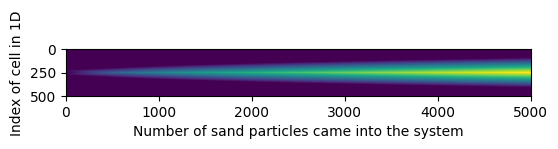
\includegraphics[width=4.3in]{pileup}
	\caption{The height of 1D as the function of time/sand particles came to system. As it can be seen, the system behaves like expected, medium locations are pretty evenly distributed, but the toppling smooths sands all over the system.}
	\label{fig:pileup}
\end{figure}

Result is just as it is expected, medium pretty evenly distributed,  but due to toppling the edges smooths up.

The dependency between sands came into system and amount of toppled is illustrated in the Figure \ref{fig:toppling}.

\begin{figure}[!hbt]
	\centering
	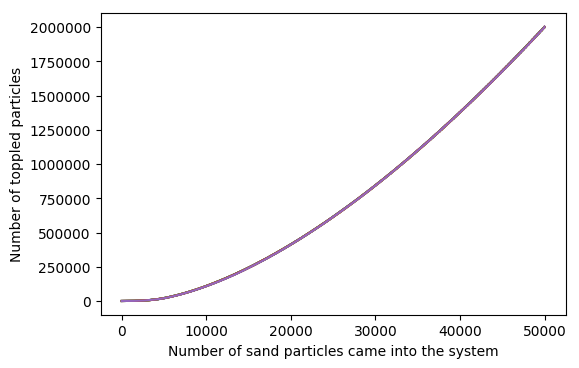
\includegraphics[width=4.3in]{toppling}
	\caption{Part 1, number of sands toppled as a function on the sands came to the system.}
	\label{fig:toppling}
\end{figure}

So large number of topplings can be explained as toppling continuing/starting from the endpoint after the previous toppling ends.


\clearpage
\subparagraph*{Part 2, generating all at once\\}

In this section all points are generated at the start, which results in a starting situation similar to Figure \ref{fig:part2starting1000points} in case of N=10000 and similar Figure \ref{fig:part2start106} in case of $10^6$ points.

The starting setup is that edge points are set to 0, so there is no boundary issues. 

The toppling rule is that if difference between connected cells is more than 2, the toppling will occur, so that the 1/3 of the difference passes to the lower cell. In case if toppling spot can topple left and right, than the lower one is chosen as toppling direction. 



\begin{figure}[!hbt]
	\centering
	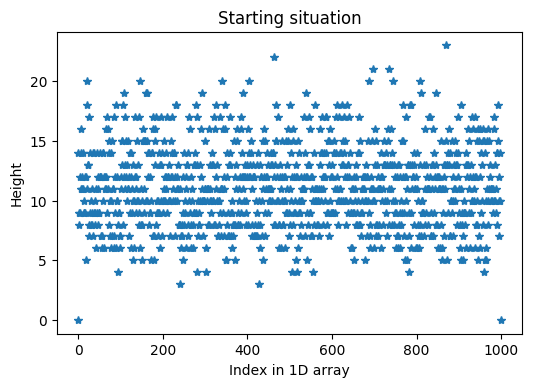
\includegraphics[width=4.3in]{part2starting1000points}
	\caption{Part 2, starting case of 10000 sands.}
	\label{fig:part2starting1000points}
\end{figure}


\begin{figure}[!hbt]
	\centering
	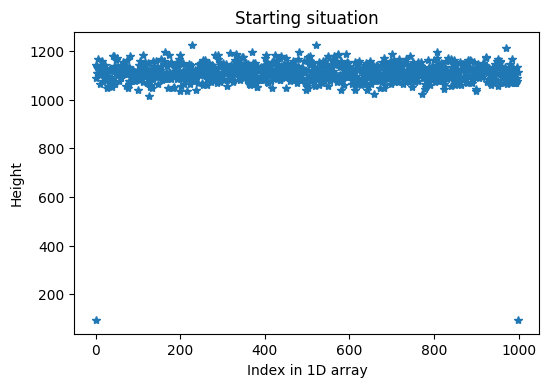
\includegraphics[width=4.3in]{part2start106}
	\caption{Part 2, starting case of 1'000'000 sands.}
	\label{fig:part2start106}
\end{figure}

Now starts the toppling, which will result in Figure \ref{fig:part2end106}

\begin{figure}[!hbt]
	\centering
	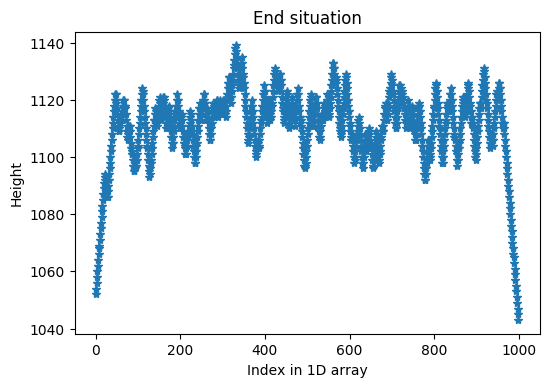
\includegraphics[width=4.3in]{part2end106}
	\caption{Part 2, ending situation in case of 1'000'000 sands. Each star is a cell.}
	\label{fig:part2end106}
\end{figure}

The N as the function of the sum of sands toppled is illustrated in Figure \ref{fig:part2sa}.

\begin{figure}[!hbt]
	\centering
	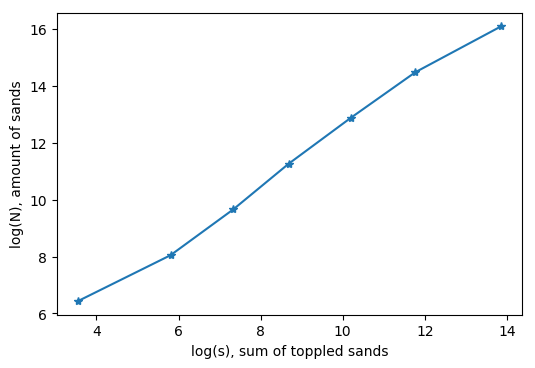
\includegraphics[width=4.3in]{part2sa}
	\caption{Part 2, log(N) and log(s).}
	\label{fig:part2sa}
\end{figure}

As it can be see the logarithmic dependency between N and s is almost a straight line. Which represents the claim presented in lecture notes that N $\propto$ $s^{something}$.


\end{document}